\chapter{Ecureuil AS-350 (semi-monocoque)}
\label{ch:Eurocopter AS350 (monocoque frame)}

\noindent
\emph{Another finite-element model regarding a modern semi-monocoque type of tailboom's design has been developed in order to compare and predict the vibration characteristics of the newer rotorcraft machines such as the Eurocopter AS-350 here presented.}

\section*{Introduction}
\addcontentsline{toc}{section}{Introduction}
\noindent
The \textbf{Eurocopter AS-350 Écureuil} is a single-engine light helicopter originally designed and manufactured in France by Aérospatiale, now Airbus Helicopters. It is widely spread for its unparalleled high-altitude capabilities and performance and has proven to be the most safe and reliable helicopter in the industry. \\
It has really close dimensions and technical specifications to the lama's helicopter and it is commonly considered its direct evolution. In fact, in the early 1970s, Aérospatiale decided to initiate a new development programme to produce a suitable replacement for the aging Aérospatiale Alouette II (Lama) for a new civil-orientated operations. \\
The development of the new rotorcraft, which was headed by Chief Engineer René Mouille, was focused on the production of an economic and cost-effective aerial vehicle, thus both Aérospatiale's Production and Procurement departments were heavily involved in the design process.
One such measure was the use of a rolled sheet structure, a manufacturing technique adapted from the automotive industry; another innovation was the newly developed Starflex main rotor. Right now, more than 3700 Ecureuil have been sold in the world overcoming millions of flying hours time.

\begin{figure}[t]
\centering
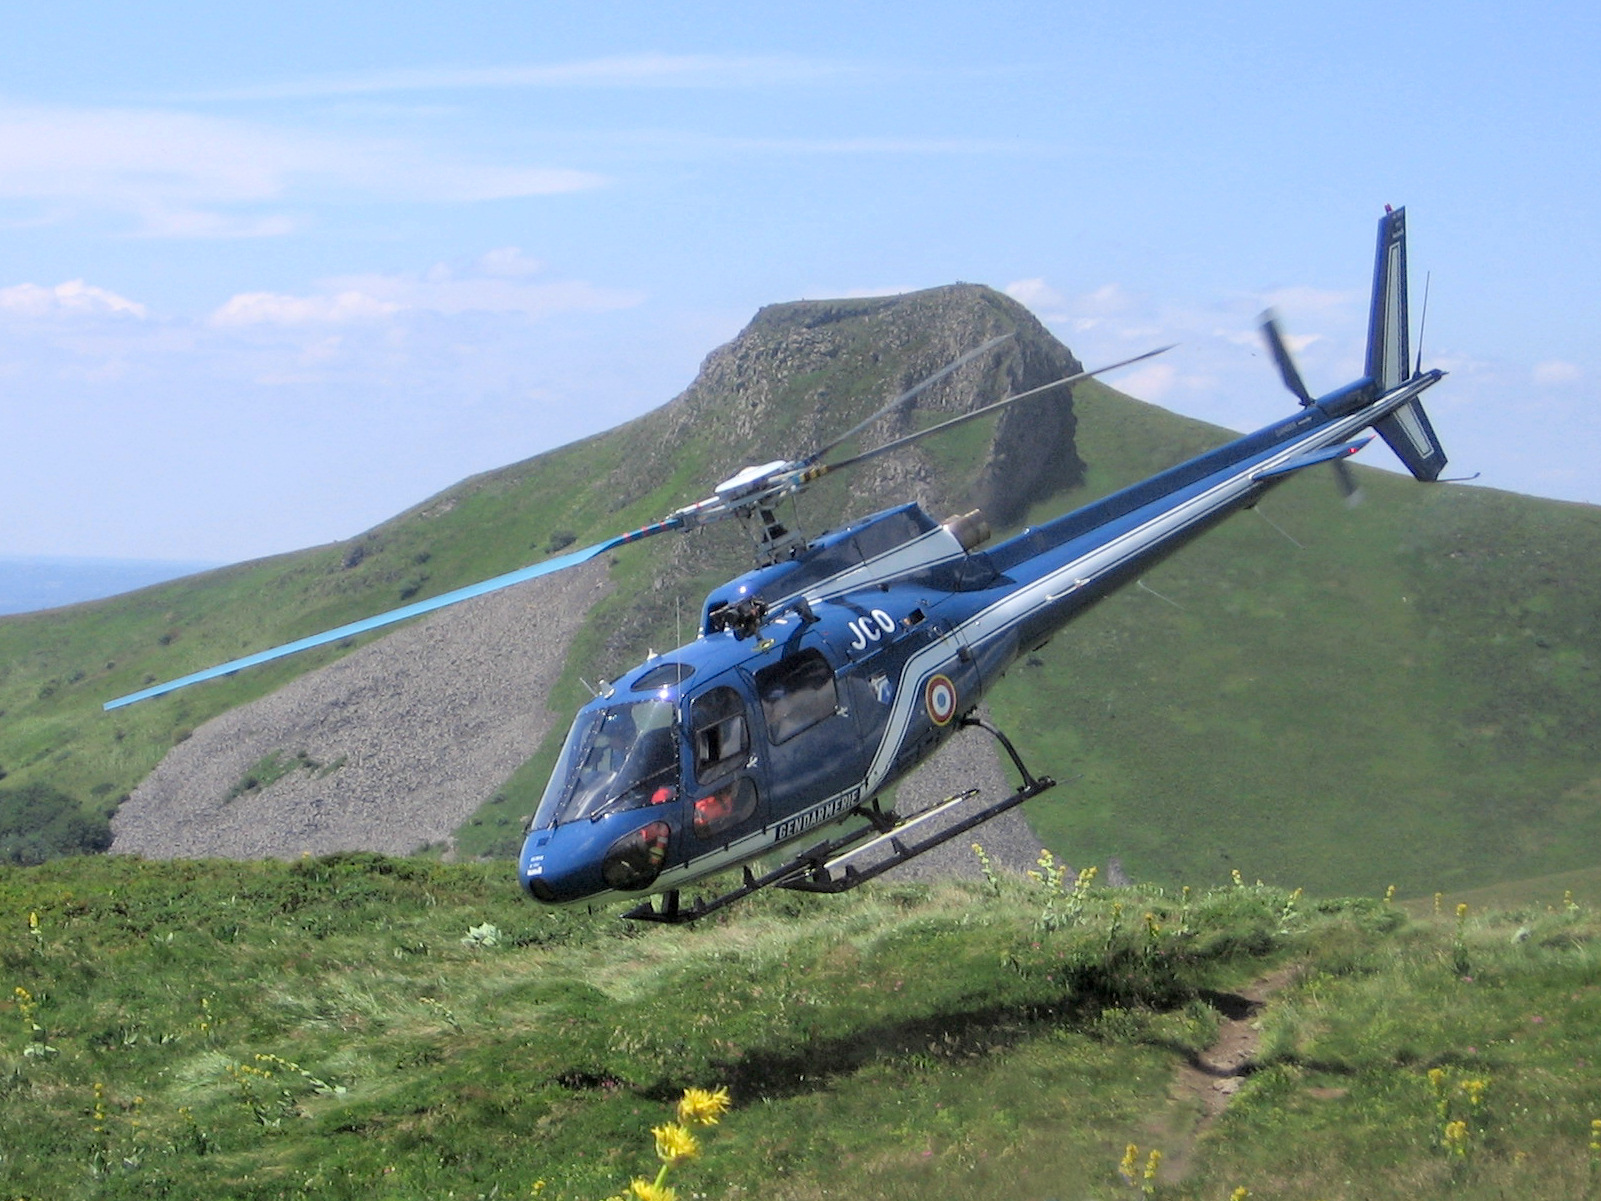
\includegraphics[width=0.80\textwidth]{imgs/Helicopter_rescue_sancy_takeoff}
\caption{Helicopter takeoff \\Di Fabien1309 - Own work}
\label{fig:AS350wiki}
\end{figure}

\begin{minipage}{\textwidth}
  \begin{minipage}[b]{0.49\textwidth}
   	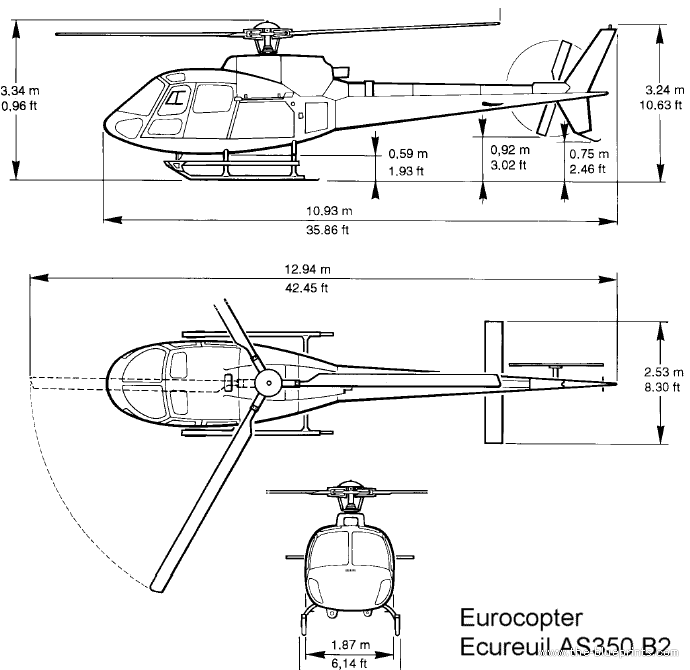
\includegraphics[width=\textwidth]{imgs/eurocopter-as350-b2}
    \captionof{figure}{AS350 blueprints\label{fig:AS350blueprints}}
  \end{minipage}
  \hfill
  \begin{minipage}[b]{0.49\textwidth}
    \centering
    \begin{tabular}{%
		>{}l%
		>{}l%
		>{\columncolor{yellow}}r}
		\multicolumn{2}{>{\columncolor{lightgray}}c}{General characteristics}\\
		Length	&	12.94 m\\
		Height	&	3.34 m\\
		Main rotor diameter& 10.69 m\\
		Empty weight		& 1220 kg\\
		Max takeoff weight & 2250 kg\\
		capability	& 2500 kg\\
		\multicolumn{2}{>{\columncolor{lightgray}}c}{Propulsion}\\
		Powerplant	&	1 x Turbine\\ 
		& Turbomeca\\& Arriel 1D1\\
		Power	&	546 kW\\
		\multicolumn{2}{>{\columncolor{lightgray}}c}{Performance}\\
		Maximum speed & 287 km/h\\
		Range	 & 476 km\\
		service ceiling 	 & 6100 m\\
    \end{tabular}
  \captionof{table}{Main characteristics AS350}\end{minipage}
\end{minipage}

\subsection*{General structural description}
\addcontentsline{toc}{subsection}{General structural description}
\noindent
The semimonocoque airframe, as introduced in chapter 1, is composed of:
\begin{itemize}
	\item longitudinal longerons;
	\item vertical formers and bulkhead; 	
	\item stringers;
	\item external skin.
\end{itemize}

\noindent
All these elements are designed to be attached together and to the skin to achieve the full strength benefits of semimonocoque design. It is important to recognize that the metal skin or covering carries
part of the load in this type of construction. \\
Furthermore, \emph{spreading loads among these structures and the skin means no single piece is failure critical and so, the fuselage may withstand considerable damage before failing}. \\

%\smallskip
\begin{figure}[h!]
	\begin{center}
		\centering  		 		
		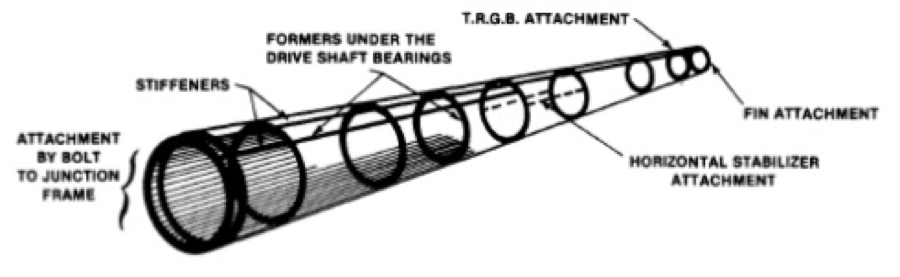
\includegraphics[width=0.9\linewidth]{PICTURES/3_Ecureuil/semimonocoque2}
	\end{center}
	\caption{Elements in a semimonocoque construction}
\end{figure}	
%\vspace{0.5cm}



\section*{Material properties}
\addcontentsline{toc}{subsection}{Material properties}
\noindent
The semimonocoque fuselage is constructed primarily of alloys of aluminum, although steel is adopted for the formers that support the drive shaft bearings and for the junction frame, attached by bolts, to the cockpit.

\begin{table}[h!]
	\centering
	
	\begin{tabular}{c c c c} 
		\toprule
		\multicolumn{4}{c}{Material properties}\\
		\midrule
		Mat & Density (kg/m3) & Poisson's ratio & Young's modulus (GPa) \\
		\midrule
		Steel & 7850  &  0.29 & 205 \\ 
		\midrule
		Aluminium & 2700  &  0.34 & 64 \\
		\bottomrule
	\end{tabular}	
\end{table}

\clearpage
\section*{Element types}
\addcontentsline{toc}{subsection}{Element types}
\noindent
The semimonocoque's model has been discretized using the following element's types:
\begin{itemize}
	\item \textbf{BEAM 189}: with rectangular cross-section to model Longerons and stringers, as shown in \ref{subfig:Rectagnle}, and with square cross-section to model stiffners \ref{fig:SectionGeometry};
	\item \textbf{SHELL 181}: to model the outer aluminium skin which compose the coverage of the structure;
	\item \textbf{MPC 184}: to rigidly connect to the airframe the concentrated masses representing the tail rotor drive shaft supported by its bearings.
\end{itemize}
%
The complete structure skeleton is represented in fig. \ref{fig:Skeleton}.
%
\bigskip
\begin{table}[h!]
	\centering
	
	\begin{tabular}{c c r l} 
		\toprule
		\multicolumn{4}{c}{Tubes cross section's properties}\\
		\midrule
		Family & Parameter & Value & Description \\
				
		\midrule
		& $length$ &  5.2 $[m]$ & Total tail length \\
		& $b \, * \, h$ &  9 x 1.5 $[mm]$ &  Cross section's dimensions\\ 
		Longerons & $A_{section}$  &  13.5 $[mm^2]$ & Area of the cross section \\ 
		& $I_{x} = I_{y}$ &  $91.125$ $[mm^4]$ & Moment of inertia \\ 
		
		
		\midrule
		& $length$ &  5.2 $[m]$ & Total length \\
		& $b \, * \, h$ &  5 * 5 $[mm]$ &  Cross section's dimensions\\ 
		Stiffners & $A_{section}$  &  25 $[mm^2]$ & Area of the cross section \\ 
		& $I_{x} = I_{y}$ &  $52.08$ $[mm^4]$ & Moment of inertia \\ 	
		
		\bottomrule
	\end{tabular}
	\caption{Structural elements characteristics}
	
\end{table}

\begin{figure}[!htb]
	\centering
	\subfloat[][\emph{Rectangular}.\label{subfig:Rectagnle}]{
		\resizebox{.25\linewidth}{!}{\begin{tikzpicture}
%linee guida
%\foreach \x in {0,1,...,15}
%   \draw [help lines] (\x,0) node [below,%
%          font=\footnotesize] {$\x$} -- (\x,15);
%%\foreach \y in {0,1,...,15}
%%   \draw [help lines] (0,\y) node [left,%
%%          font=\footnotesize] {$\y$} -- (15,\y);

\node at (1,14) (a) {};
\node at (3,14) (b) {};
\node at (3,10) (c) {};
\node at (1,10) (d) {};

\draw (a) rectangle (c);
\draw[-latex] (2,12)--( 2,9.5)node[right]{\scriptsize x};
\draw[-latex] (2,12)--(3.5,12)node[above]{\scriptsize y};


% quote track
 \dimline    [color=gray,
 			  label style={above=0.1ex},
                % line style={thick},
                %extension start style={gray,thin},
                %extension end style={gray,thin},
                extension start length=0.5cm,
                extension end length=0.5cm
                ]{(1,14.5)}{(3,14.5)}{$b$};
                
\dimline    [color=gray,
                % line style={thick},
                %extension start style={gray,thin},
                %extension end style={gray,thin},
                extension start length=0.5cm,
                extension end length=0.5cm
                ]{(0.5,10)}{(0.5,14)}{$w$};
\end{tikzpicture}}} \quad
	\subfloat[][\emph{Square}.\label{subfig:Square}]{
		\resizebox{.25\linewidth}{!}{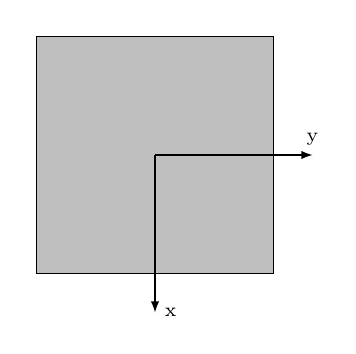
\begin{tikzpicture}
%linee guida
%\foreach \x in {0,1,...,15}
%   \draw [help lines] (\x,0) node [below,%
%          font=\footnotesize] {$\x$} -- (\x,15);
%\foreach \y in {0,1,...,15}
%   \draw [help lines] (0,\y) node [left,%
%          font=\footnotesize] {$\y$} -- (15,\y);

\node at (1,14) (a) {};
\node at (4,14) (b) {};
\node at (4,11) (c) {};
\node at (1,11) (d) {};

\draw[fill=lightgray] (a) rectangle (c);
\draw[-latex] (2.5,12.5)--( 2.5,10.5)node[right]{\scriptsize x};
\draw[-latex] (2.5,12.5)--(4.5,12.5)node[above]{\scriptsize y};


% quote track
 \dimline    [color=gray,
 			  label style={above=0.1ex},
                % line style={thick},
                %extension start style={gray,thin},
                %extension end style={gray,thin},
                extension start length=0.5cm,
                extension end length=0.5cm
                ]{(1,14.5)}{(4,14.5)}{$5$};
                
\dimline    [color=gray,
			label style={above=0.1ex},
                % line style={thick},
                %extension start style={gray,thin},
                %extension end style={gray,thin},
                extension start length=0.5cm,
                extension end length=0.5cm
                ]{(0.5,11)}{(0.5,14)}{$5$};
\end{tikzpicture}}}\\
	\caption{Section for element \textsc{beam189}}
	\label{fig:SectionGeometry}
\end{figure}

\clearpage
\section*{Approach to the problem}
\section{Geometric model (airframe only)}
\subsection*{Analysis model}
\addcontentsline{toc}{subsection}{Analysis model}

\noindent
We approached this problem with the same steps of the previous helicopter's tail model. Firstly only the naked airframe has been studied considering it just as a cantilever beam, then, subsystems have been added to increase the accuracy of the model adding the drive shaft (considered as distributed masses along the tail's length) and other concentrated masses and inertias to represent the tail rotor assembly at the tail's tip. \\

\noindent
The created model can be seen in the figure \ref{fig:AnsysMeshLump}.

\medskip
\begin{figure}[h!]
	\begin{center}
		\centering  		 		
		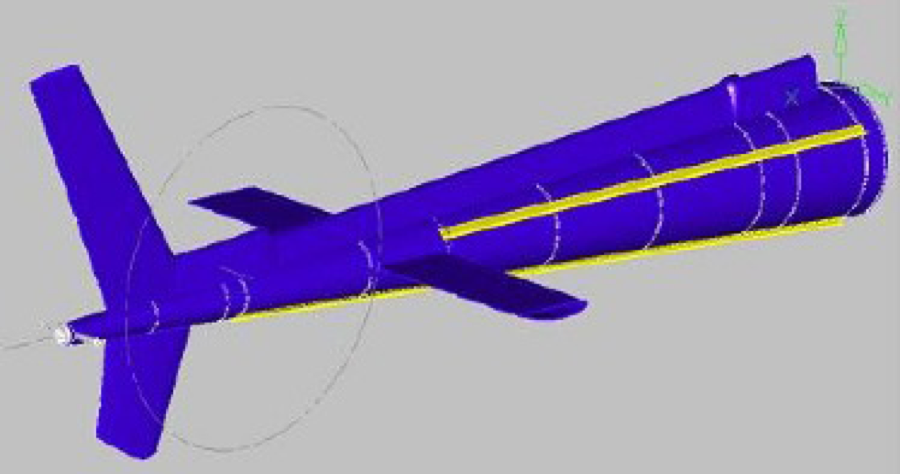
\includegraphics[width=0.8\linewidth]{PICTURES/3_Ecureuil/analysis_model}
	\end{center}
	\caption{Analysis model}
\end{figure}	
%\vspace{0.5cm}

\medskip
\begin{table}[h!]
	\centering
	
	\begin{tabular}{c c r l} 
		\toprule
		\multicolumn{4}{c}{Tubes cross section's properties}\\
		\midrule
		Family & Parameter & Value & Description \\
		\midrule
		& base radius &  \textbf{325} $[mm]$ & Base radius (cone) \\
		& top radius &  \textbf{50} $[mm]$ & Top radius (cone) \\
		Model dimensions & tail length &  \textbf{5.2} $[m]$ & Total tail length \\
		& 7 segments &  \textbf{0.74} $[m]$ & Total segment length \\
		& skin thickness &  $\textbf{0.5}$ $[mm]$ & Shell thickness \\
		\bottomrule
	\end{tabular}
	\caption{Tailboom's model dimensions}
	
\end{table}


\clearpage
\subsection*{Model assumptions}
\addcontentsline{toc}{subsection}{Model assumptions}

\noindent
\begin{quoting}
	\begin{itemize}
		
		\item Element type: \textbf{BEAM 189} based on Timoshenko beam theory which includes shear-deformation effects and \textbf{SHELL 181} elements to discretize the structure;
		
		\item uniform cross-sections of the elements and of the shell thickness along the tail's length;
		
		\item riveting and bolting connections of the coverage skin not considered;
		
		\item \underline{linear elastic isotropic} material properties;
		
		\item self-weight of the elements considered;
		
		\item geometrical non-linearities included in the static analysis (NLGEOM,ON) \\
		
	\end{itemize}
\end{quoting}

\smallskip
\subsection*{Tailboom geometric model (airframe only)}

\begin{figure}[!htb]
	\centering
	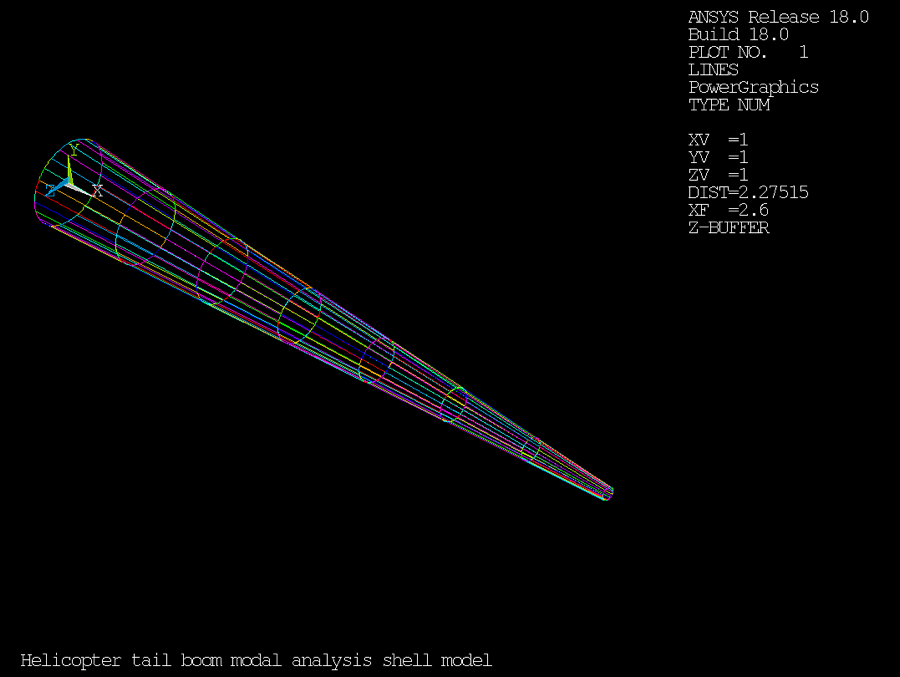
\includegraphics[width=0.75\textwidth]{PICTURES/imgs/ShellModel/img/Shellmodel000.png}
	\caption{Model geometry (isometric view)}
	\label{fig:Geometric}
\end{figure}


\begin{figure}[!htb]
	\centering
	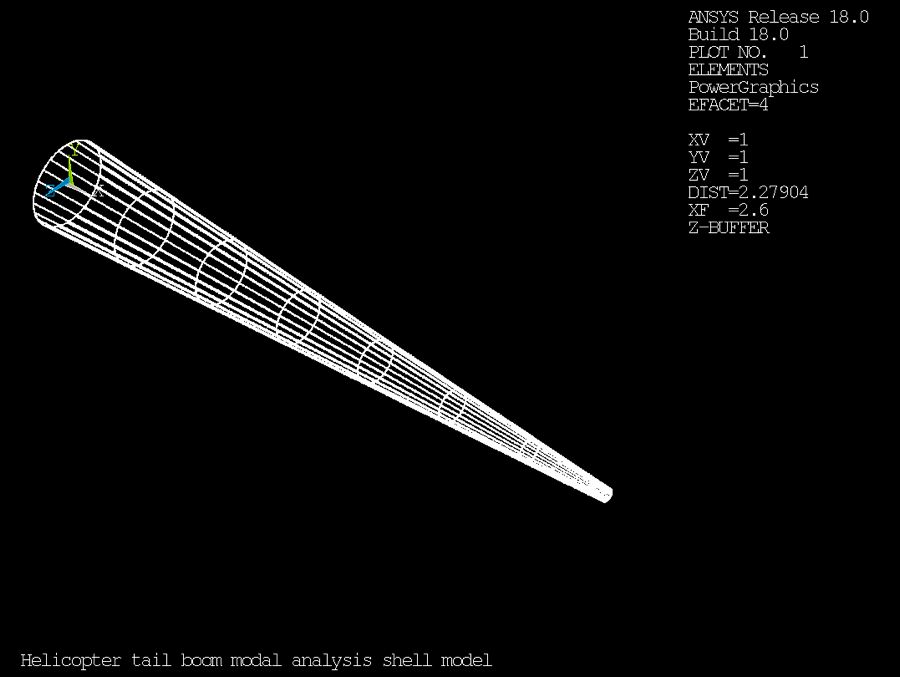
\includegraphics[width=0.75\textwidth]{PICTURES/imgs/ShellModel/img/Shellmodel001.png}
	\caption{Tailbooms skeleton (isometric view)}
	\label{fig:Skeleton}
\end{figure}



\subsection*{Aluminium's outer skin}
\noindent
The outer skin which represents the external coverage of the airframe and which contributes to support part of the external load has been modelled using SHELL 181 elements of constant thickness. 
Riveting connections have not been modelled for simplicity.
%
\begin{figure}[!h]
	\centering
	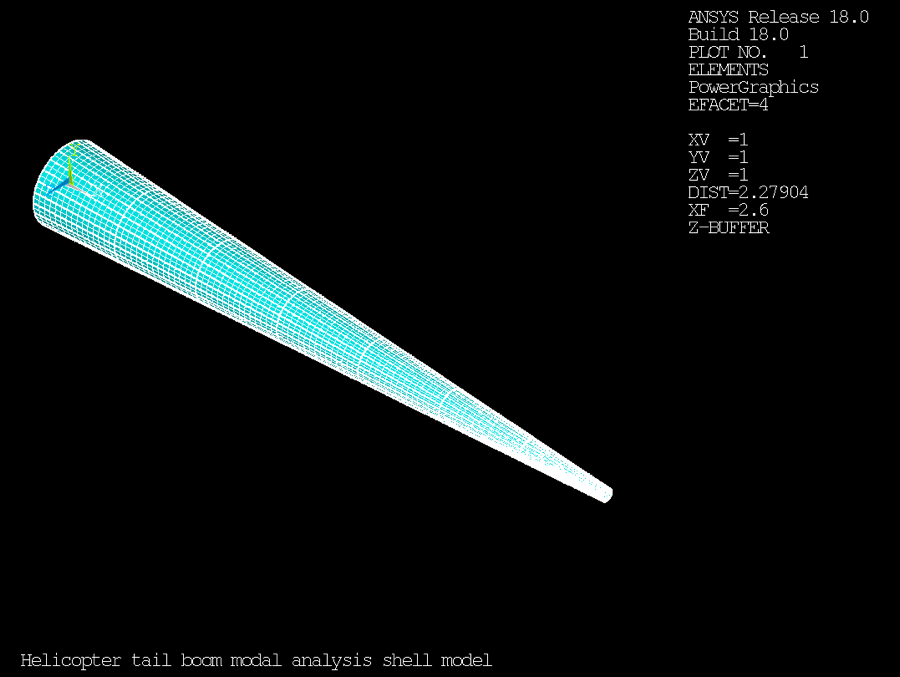
\includegraphics[width=0.75\textwidth]{PICTURES/imgs/ShellModel/img/Shellmodel002.png}
	\caption{Aluminium's outer skin}
	\label{fig:AnsysMeshLump}
\end{figure}
%
\subsection*{Applied loads and boundary conditions}
\addcontentsline{toc}{subsection}{Applied loads and boundary conditions}
\noindent
The loads considered for the static analysis are exactly the same of the previous model, but the force is applied at the rotor hub's attaching point which, in this case, is not at the tail tip but at a point near the rear end. \\
For the boundary conditions, again the tail is considered as a cantilever beam but this time the all nodes of the base junction have been constrained to the ground. \\


\section{Preliminary static analysis}
\noindent
As we saw before, the preliminary static analysis is performed in such a way to check if the all structure is well posed and ready for the modal analysis.
So, we have looked into the deformation caused by the self-weight of the structure, due to the gravity acceleration, and to the tail rotor thrust force. 



\subsubsection*{PLDISP and PLNSOL (node's displacement)}
%\smallskip
\begin{figure}[h!]
	\begin{center}
		\centering  		 		
		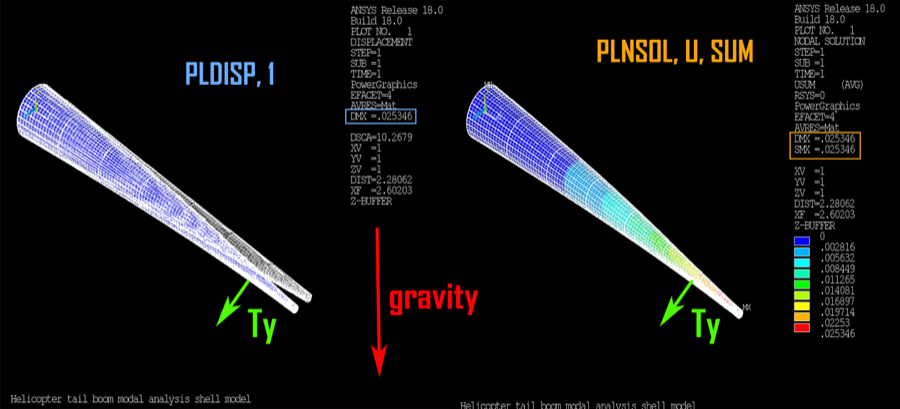
\includegraphics[width=0.95\linewidth]{PICTURES/3_Ecureuil/static_analysis_simple.png}
	\end{center}
	%\caption{Model's boundary conditions}
\end{figure}	
%\vspace{0.5cm}

\noindent As a matter of fact, we can observe that this value (maximum displacement) 
compared among both models is very closed each other. We can also prove that shell model is more flexible than the truss model, as a consequence of a bigger total displacement.\\
Furthermore it is evident that in the normal operation the tailboom is \textbf{pre-loaded} by the aerodynamic thrust force provided by the tailrotor. This pre-load as an effect on the vibrational behaviour of the system. 



\clearpage
\section*{Modal Analysis (airframe only)}
\addcontentsline{toc}{subsection}{Modal Analysis (airframe only)}
\noindent
After a mesh refinement and a convergence analysis, the first 20 values of the natural frequencies of the shell monocoque airframe have been extracted and are now listed in the following table:

\begin{table}[h!]
	\centering
	\pgfplotstableset{
		% global config, for example in the preamble
		% these columns/<colname>/.style={<options>} things define a style
		% which applies to <colname> only.
		every head row/.style={before row=\hline,after row=\hline},
		every last row/.style={after row=\hline},
		display columns/0/.style={column name =Mode, int detect,column type=r},
		display columns/1/.style={column name =Frequence [Hz], column type=r,
			fixed,fixed zerofill,precision=5,set thousands separator={\,}},
		%other style option   
	}
	\pgfplotstabletypeset[col sep=space]{ModalFreq-Shellmodel.txt}
	\caption{Natural frequencies for the simple model}
	\label{tab:ModalFreq-Shellmodel}
\end{table}


\bigskip
\noindent
IMPORTANT NOTE: \\
The applied boundary conditions (fixed - free) constrain the structure in order to be \textbf{statically determinate}. In fact, NO zero-frequency modes have been found, as it can be seen in the table 3.4.
So, the stiffness matrix of our structure, thanks to the type of the constraint, results to be \textbf{positive definite} and NO rigid motions of the system occur. \\




\clearpage
\section{Full shell model (airframe + subsystems)}

\noindent
Starting from the simple airframe model, concentrated masses with rigid links are added to represent the aircraft subsystems in a lumped formulation. \\ The element used is the well known \textsc{mass21} with mass and inertia concentrated properties. This introduce an approximation in the analysis of the structure but it allows it to be simpler and computationally lighter to be solved. \\
In the following picture, the components we intend to model are shown on a real Ecureil helicopter type: \\ 


\begin{figure}[h!]
	\begin{center}
		\centering  		 		
		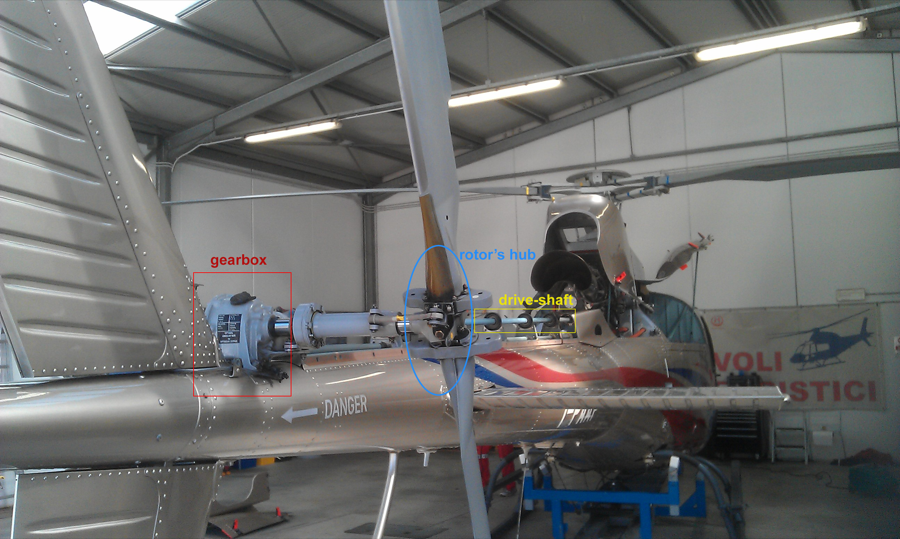
\includegraphics[width=1\linewidth]{PICTURES/3_Ecureuil/IMAG0112.png}
	\end{center}
	\caption{Drive-shaft, gearbox and rotor assembly parts}
\end{figure}	
\vspace{0.5cm}


\noindent
In order to ensure rigid connections between the concentrated masses and the airframe structure, elements of type: \textsc{mpc184}, with key option: $1$, are used to block six degrees of freedom for each element. \\

\noindent
The gearbox is attached in the rear three-quarter of the tailboom and considered again as a lumped mass by using the element type \textsc{mass21} located on the last bearing node. \\

\clearpage
\medskip
\noindent
The following list contains the values of the concentrated masses considered in the model:

\begin{itemize}
	\item drive shaft total mass: $12\,[kg]$ divided on the 7 support bearings along the tail;
	\item gearbox concentrated mass: $30\,[kg];$
	\item rotor assembly: $15\,[kg];$
\end{itemize}

\medskip
\begin{figure}[h!]
	\begin{center}
		\centering  		 		
		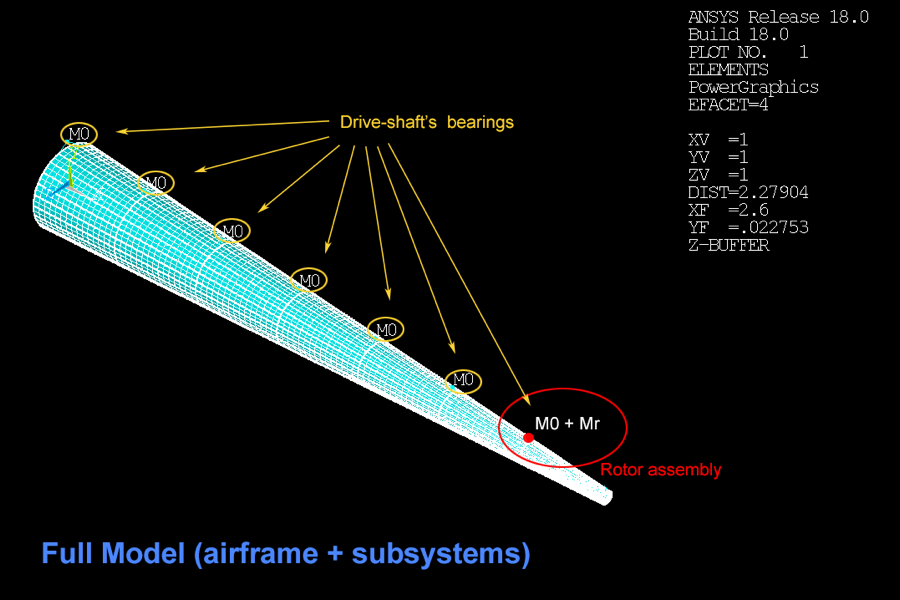
\includegraphics[width=0.95\linewidth]{PICTURES/3_Ecureuil/full_model.png}
	\end{center}
	\caption{Complete shell model ready for the modal analysis.}
\end{figure}	
\vspace{0.5cm}




\clearpage
\section*{Modal Analysis (full tail model)}
\addcontentsline{toc}{subsection}{Modal Analysis (full tail model)}
\noindent

\noindent
After a mesh refinement and a convergence analysis, the first 20 values of the natural frequencies of the shell semi-monocoque airframe have been extracted and are now listed in the following table \ref{ModalFreq-ShellmodelShaftLumped}:

\begin{table}[!h]
	\centering
	\pgfplotstableset{
		% global config, for example in the preamble
		% these columns/<colname>/.style={<options>} things define a style
		% which applies to <colname> only.
		every head row/.style={before row=\hline,after row=\hline},
		every last row/.style={after row=\hline},
		display columns/0/.style={column name =Mode, int detect,column type=r},
		display columns/1/.style={column name =Frequence [Hz], column type=r,
			fixed,fixed zerofill,precision=5,set thousands separator={\,}},
		%other style option   
	}
	\pgfplotstabletypeset[col sep=space]{ModalFreq-ShellmodelShaftLumped.txt}
	\caption{Natural frequencies for the model with lumped mass}
	\label{ModalFreq-ShellmodelShaftLumped}
\end{table}%

\bigskip
\noindent
IMPORTANT NOTE: \\
\noindent
As before, those resonant frequencies are computed without considering the tail-rotor rotation.
The \emph{tailrotor-fuselage coupling} will be introduced in the next chapter.

\clearpage

\subsection*{Modal shapes}
\noindent
Eigenvectors are typically normalized in Ansys with respect to the mass matrix and; this normalization is very useful from the computational point of view. However, the drawback is that in this way they represent correctly the shape of the mode but not the real amplitude of the displacement which in turn depends on the initial conditions. 

\begin{figure}[h]
	\begin{center}
		\centering  		 		
		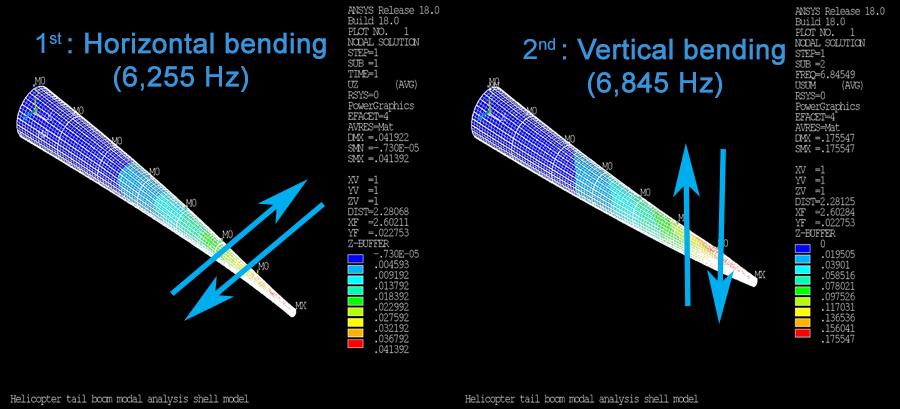
\includegraphics[width=0.95\linewidth]{PICTURES/3_Ecureuil/1-2.png}
	\end{center}
	\caption {Graphical representation of the first and second modal shapes}
\end{figure}

\noindent
The first three mode shapes are related to the \emph{horizontal,vertical and torsional} movement of the tailboom. The last one shows the shell expansion effect. 

\begin{figure}[h]
	\begin{center}
		\centering  		 		
		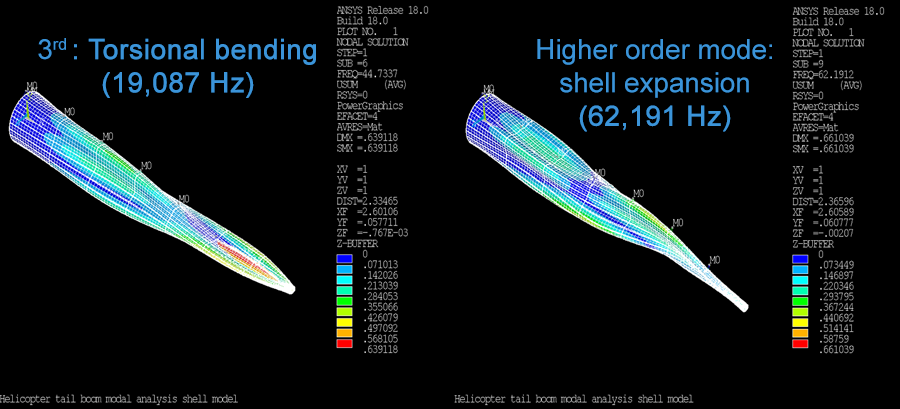
\includegraphics[width=0.95\linewidth]{PICTURES/3_Ecureuil/3-4.png}
	\end{center}
	\caption {Graphical representation of higher order modal shapes}
\end{figure}
